\documentclass[tikz,border=0pt]{standalone}

\usepackage{graphicx}
\usepackage{amsmath}
\usepackage{xcolor}

\definecolor{surgery_image_red}{HTML}{C93517}
\definecolor{surgery_image_blue}{HTML}{36A9E1}
\definecolor{surgery_image_green}{HTML}{009640}

\begin{document}

\begin{tikzpicture}
    \node[anchor=south west, inner sep=0] at (0,0) {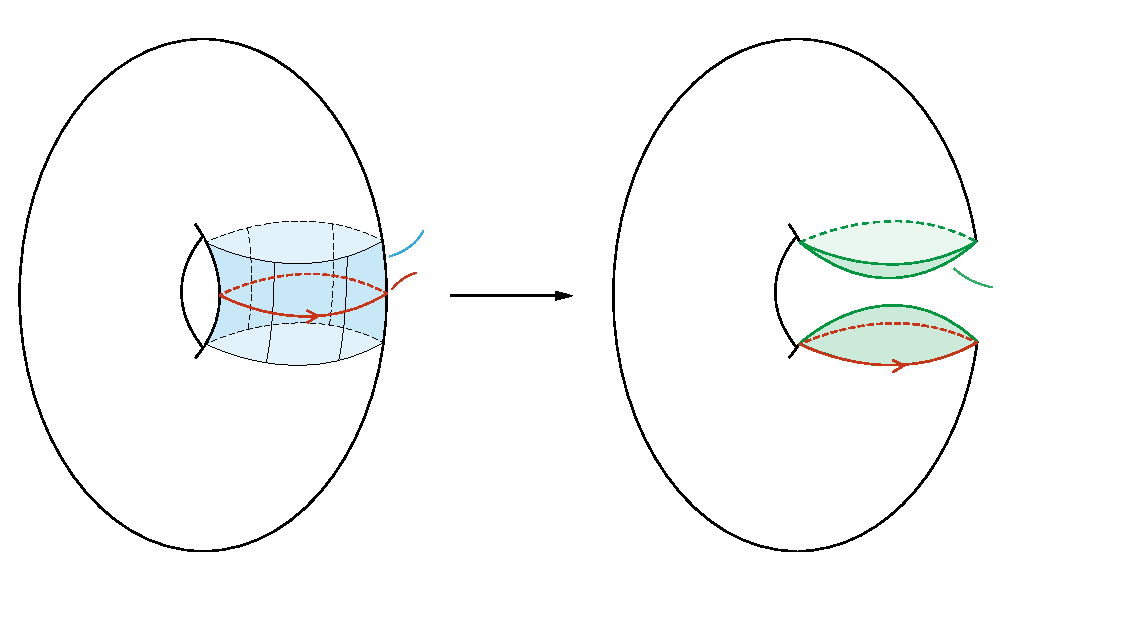
\includegraphics[trim = .1cm 1cm 1cm .5cm, clip]{surgery_raw.pdf}};

    \node at (7.7,6) {\color{surgery_image_blue}\large $\mathrm{im}(F)$};
    \node at (7.2,5.1) {\color{surgery_image_red} \large$f$};
    \node at (17.55,4.85) {\color{surgery_image_blue}\large $D^{2} \times S^{0}$};

\end{tikzpicture}

\end{document}

